%===================================== CHAP 2 =================================
\cleardoublepage

\chapter{Theory} \label{chap:3}

This chapter presents the theory on CBR methodology and CBR Recommender Systems (CBR-RS), which were used to create Utsida. It also introduces myCBR; the software tool used to model and implement the CBR-RS part of Utsida. 

\section{Case-based Reasoning}

Case-Based Reasoning (CBR) is a methodology in the field of AI for solving problems and is primarily based on experiences, i.e., the solutions of similar problems. The CBR methodology utilizes these experiences to yield solutions to a large range of problems where uncertainty is involved \cite{richter2013case}. Implied by the name, CBR can be broken down into two main concepts: \textit{cases} and \textit{reasoning}. A case is an experience of a solved problem and consists of two parts: a problem description and a solution to the problem. Reasoning refers to the approach of finding solutions to problems by evaluating different experiences (i.e. cases). Reasoning in CBR differs from other kinds of reasoning because it does not lead from true assumptions to true conclusions \cite{richter2013case}. This means that for two cases with similar problem descriptions, the solution to one of them might not be the solution to the other. The recorded experience in the first instance may not be exactly similar to the other case.
    
\subsection{Case Representation}\label{sec:feature_vectors}
A case is usually represented as a feature vector, consisting of pairs of attributes and their values. An example is a diagnosis of a sick patient, as shown in Table \ref{tab:example_case}. Here, the attributes of the case are a collection of symptoms, and the values are whether the patient has the symptom or not. The solution to the case is the final diagnosis of the patient. A \textit{Concept} is a term used for the combination of the case representation, a designated similarity measure and a weight value for each attribute in the case-representation, as well as a summation function.

\begin{table}[h]
\centering
\caption{Case representation example}
\label{tab:example_case}
\begin{tabular}{|l|l|l|}

\hline
 \textbf{Part} & \textbf{Attribute} & \textbf{Value} \\ \hline \hline
\multicolumn{1}{|l|}{\multirow{6}{*}{Problem}} & Nausea & Yes \\ \cline{2-3} 
\multicolumn{1}{|l|}{} & Fever & Yes \\ \cline{2-3} 
\multicolumn{1}{|l|}{} & Malaise & Dizzy \\ \cline{2-3} 
\multicolumn{1}{|l|}{} & Blood pressure & Normal \\ \cline{2-3} 
\multicolumn{1}{|l|}{} & Vision changes & No \\ \cline{2-3} 
\multicolumn{1}{|l|}{} & Shortness of breath & No \\ \hline
\multicolumn{1}{|l|}{Solution} & Diagnosis & Influenza \\ \hline
\end{tabular}
\end{table}

\subsection{The CBR-Cycle}\label{sec:cbr-cycle}

Aamodt and Plaza \cite{aamodt1994case} defined a model which explain the problem solving cycle in CBR (fig. \ref{fig:cbr_cycle}). The cycle defines the four distinct steps, the 4 R's, of the CBR process and can be summarized as followed.

\begin{description}
\item [1. Retrieve:] The most similar case is retrieved from the system's case-base so that it can be compared to a new case.
\item [2. Reuse:] The solution to the retrieved case is applied to the new case.
\item [3. Revise:] The new case is evaluated and tested for success, and is repaired if it fails.
\item [4. Retain:] The new case with the given solution is retained in the case base for future usage.
\end{description}

\begin{figure}[h]
    \centering
    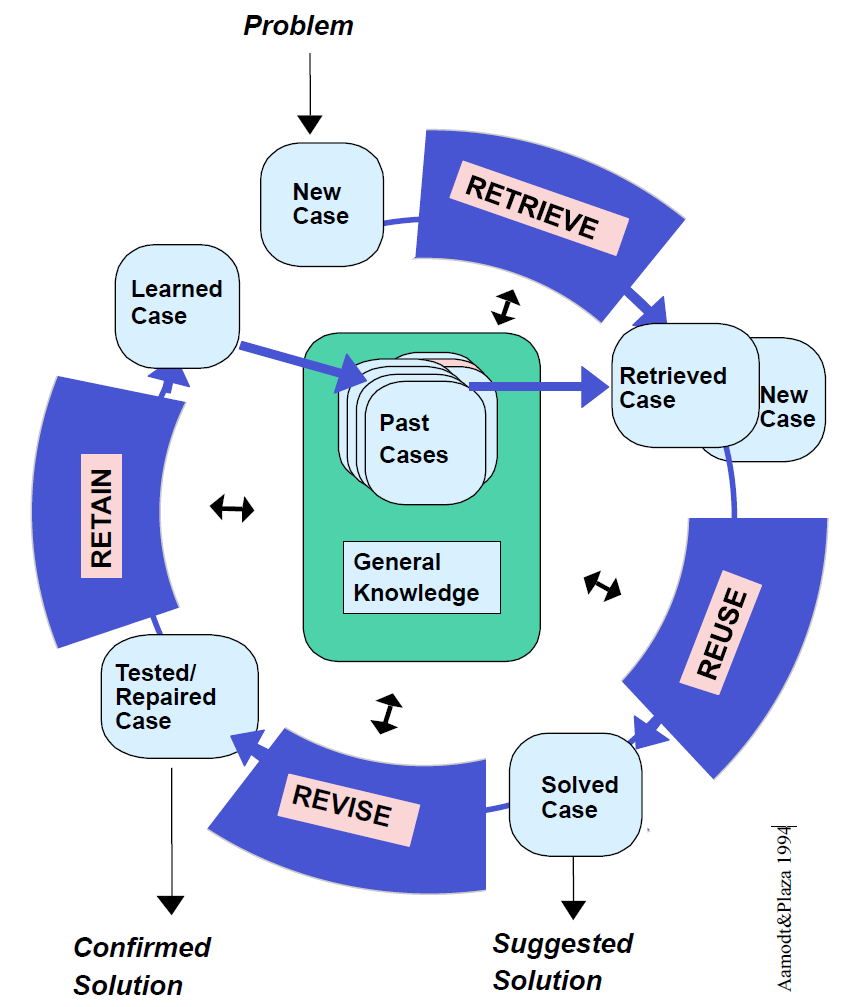
\includegraphics[width=0.6\textwidth]{fig/cbr-cycle.png}
    \caption[The CBR Cycle]{The CBR Cycle (Aamodt \& Plaza) \cite{aamodt1994case}}
    \label{fig:cbr_cycle}
\end{figure}

\subsection{Case-based Reasoning Systems}

A case-based reasoning System (CBRS) is a system which use the CBR methodology to solve problems. When the system receives a new problem, it first performs step 1 in the CBR-cycle (retrieve). This step includes using similarity measures to determine the similarity between each case and the new problem. Next, the system selects the most similar case and applies and adapts the solution of this case to the new problem (step 2, reuse). The proposed solution to the new problem is tested by the system, and if found necessary, repaired (step 3, revise). Finally, the adapted solution is stored as a new case in the system's collection of cases, called the case-base (step 4, retain).

\subsection{Similarity Measures}

Similarity measures calculate the degree of similarity (i.e. similarity score) between an attribute in a problem and the corresponding attribute in a case from the case-base. The similarity measure for each attribute is usually different and is often tailored to suit the data type of the attribute, e.g. integer, string or symbol. Each attribute in a case also has a weight value, which decides the importance of that attribute. The total similarity between a case and a problem is commonly calculated by using a summation function on the similarity scores with the weights as coefficients.

\section{myCBR}

myCBR\footnote{myCBR: \url{http://www.mycbr-project.net/}} is a tool for rapid prototyping of CBRSs and focuses on the retrieval step of the CBR cycle \cite{Stahl2008}. It is developed and maintained as a joint project between the German Research Center for Artificial Intelligence and the School of Technology and Computing at the University of West London. The myCBR project includes two parts: a Software Development Kit (SDK), and a graphical user interface (GUI) called the myCBR Workbench.

The myCBR SDK is written in the Java programming language and is the core of myCBR, containing all of its functionality. The SDK allows developers to use or extend the functionality of myCBR in custom applications. The current version (3.1) of the myCBR SDK only supports the similarity based retrieval step of the CBR-cycle.

The myCBR Workbench provides a GUI for implementing and modeling most of the functionality in the SDK. The GUI lets developers prototype and utilizes the SDK without having an in-depth knowledge of its inner functions. The myCBR Workbench supports importing predefined cases with the Comma-separated values (CSV) file format. It also includes a set of default similarity measures, which are visualized with graphs and tables, making modeling of concepts easier.

\section{Case-based Reasoning Recommender Systems}\label{sec:case_based_recommender_systems}

Recommender systems mainly use either a collaborative or case-based approach to give recommendations \cite{bridge2005case}. The collaborative approach uses the rating and opinions of other users who have experienced a product or gone through the same process. The case-based approach, on the other hand, uses a case-base as the pool of information to pick recommendations from.

A case-based reasoning recommender system (CBR-RS) share many similarities with case-based reasoning systems (CBRS). The most noteworthy is that both types of systems have a case-base which they use to determine the best solution or recommendation. While a CBRS receives a query structured as a problem, a CBR-RS, on the other hand, receives a query structured more like a wish \cite{richter2013case}. This wish includes user preferences and, if present, information from a user profile. The main difference between the two systems, however, lies in the way the systems propose a solution to a query. A CBR-RS usually gives several recommendations relevant to the wish of the user, while a CBRS typically gives a single solution which matches the query best. Similar to a CBRS, a CBR-RS use CBR as the underlying methodology. The use of similarity-based retrieval is a beneficial feature for both CBR-RS and CBRS, giving advantages compared to more traditional exact matching techniques such as conventional database retrieval and classical constraint satisfaction techniques \cite{bridge2005case}.

\section{Evaluating Recommender Systems}

Recommendation systems are often evaluated and ranked based on their prediction power \cite{shani2011evaluating}. However, what is considered a relevant recommendation in a given scenario is often subjective. Therefore, it is challenging to evaluate whether a recommendation is satisfactory. For example, some users are interested in receiving recommendations which they are familiar with, while others may want recommendations that are more diverse to discover new items. Shani and Gunawardana \cite{shani2011evaluating} describes three levels of experiments to evaluate recommendation systems: offline experiments, user studies and online evaluation.

\paragraph{Offline Experiments} When evaluating recommender systems with offline experiments, there are no actual users. Instead, a collection of data based on earlier user choices is used to simulate real user queries. The results of the queries can be used to evaluate the prediction power of the recommender. The queries should, to produce proper results, be similar to the queries that users will make in a production version of the system. Since an offline experiment requires no user interaction, it is a cheap and efficient approach of evaluating a recommendation system. It does however only evaluate a small set of possible user queries, and does not provide any information on user behavior of the system.  An offline experiment can be used on different recommendation algorithms to evaluate them against each other. The data sets used to simulate user queries can either be designed by hand or by using a random selector on stored queries. Different types of biases can be introduced when generating the user queries, but methods such as reweighting or resampling can lower the influence of these biases. 

\paragraph{User Studies} In a user study the recommender system is tested on real users who are given tasks to complete. Their behavior and their satisfaction with the recommendations are then measured, and the feedback used to improve the system. User studies can use questionnaires to get feedback from users on their experience. The main advantages of a user study are that a broad range of questions can be answered and that a large amount of data, both qualitative and quantitative can be collected. The test users should represent the actual population of desired users, or else the results might be more vulnerable to biases such as non-response bias.

\paragraph{Online Evaluation} This test method allows real behavior and user interaction data to be collected from a live system. Several measures can be used to evaluate the system in an online evaluation, e.g., using different recommendation algorithms and measuring their use. To ensure a fair test of the different algorithms it is important that the users are redirected to each algorithm randomly. When the focus is only on evaluating the user interaction and design of the system, it might be more desirable to use only one algorithm and reduce the users' disorientation. 

\cleardoublepage